\documentclass[10pt,twocolumn]{article}
\pdfoutput=1
\usepackage[a4paper,margin=22mm]{geometry}
\usepackage{amsmath,booktabs,graphicx,natbib,hyperref}
\title{Reliable Optimization in Practice}
\author{TeXGlot Example Project}
\date{}
\begin{document}
\maketitle
\begin{abstract}
This reproducible example studies a simple optimization procedure. It tests a multi-file project with a vector figure, bibliography, and a two-column layout.
\end{abstract}
\section{Introduction}
Optimization algorithms are central to modern machine learning. We distinguish the \textbf{mathematical update rule} from its practical implementation, and evaluate both convergence and computational cost.

The reported error decreases from 0.25 to 0.12 after 100 steps. This comparison only illustrates how numerical results should be preserved during translation. The experiment can be repeated with a different learning rate.

\begin{figure}[t]
\centering
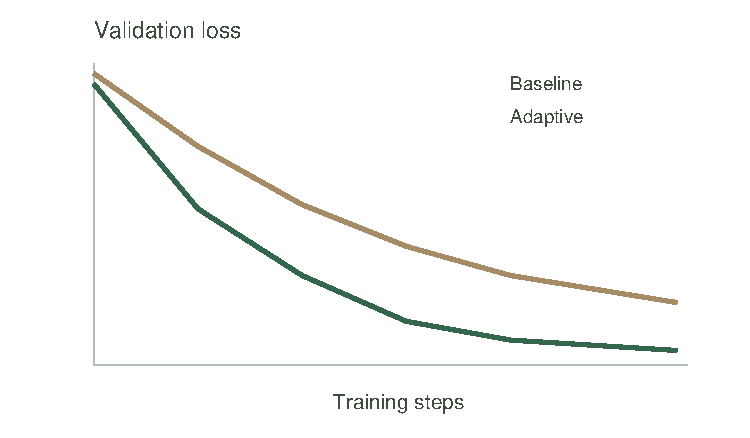
\includegraphics[width=\linewidth]{figures/convergence.pdf}
\caption{Illustrative convergence curves. The values are synthetic and do not represent a real experiment.}
\label{fig:convergence}
\end{figure}
\section{A simple update rule}
The parameters are updated by $\theta_{t+1}=\theta_t-\eta\nabla f(\theta_t)$. Here $\eta$ is the learning rate. Figure~\ref{fig:convergence} illustrates the expected trend. Standard adaptive methods provide a useful point of comparison~\citep{kingma2014}.
\begin{table}[h]
\centering
\begin{tabular}{lrr}
\toprule
Method & Error & Steps\\
\midrule
Baseline & 0.25 & 100\\
Adaptive update & 0.12 & 100\\
\bottomrule
\end{tabular}
\caption{A small numerical example.}
\end{table}
\bibliographystyle{plainnat}
\bibliography{references}
\end{document}
